\documentclass[conference]{IEEEtran}

\usepackage{amsmath,amssymb}
\usepackage{graphicx}
\usepackage{booktabs}
\usepackage{array}
\usepackage{cite}
\usepackage{url}
\usepackage{xcolor}
\usepackage{enumitem}

\graphicspath{{figures/}}
\setlength{\textfloatsep}{8pt plus 2pt minus 2pt}
\setlength{\floatsep}{8pt plus 2pt minus 2pt}
\setlength{\intextsep}{8pt plus 2pt minus 2pt}

\newcommand{\ZoneErr}{\mathrm{ZoneErr}}
\newcommand{\argmaxop}{\operatorname*{arg\,max}}
\newcommand{\argminop}{\operatorname*{arg\,min}}

\begin{document}

\title{Two-Stage Hard-Constrained WMU Placement for Fault Detection and Zone Localization under IBR-Induced Oscillatory Backgrounds}

\author{%
\IEEEauthorblockN{Hjin}
\IEEEauthorblockA{Department of Electrical and Electronic Engineering\\
Hanyang University\\
Email: 271123352+hjinyy@users.noreply.github.com}
}

\maketitle

\begin{abstract}
The increasing penetration of inverter-based resources (IBRs) introduces oscillatory background conditions that can complicate waveform-based fault monitoring. At the same time, non-fault switching events such as load switching should not trigger protection-oriented fault decisions. This paper proposes a two-stage waveform measurement unit (WMU) placement framework that separates fault detection from fault-zone localization. Stage 1 uses a hard-constrained detection anchor WMU and requires zero normal false positives, zero LoadSwitch false positives, zero single-line-to-ground fault false negatives, and zero three-phase fault false negatives. Stage 2 is activated only after a fault decision and localizes the fault to a predefined topology zone using a physically interpretable current-disturbance argmax rule. A modified IEEE 30-bus deterministic waveform dataset with IBR-like 25 Hz subsynchronous oscillation background, normal cases, 5\%, 15\%, and 30\% LoadSwitch cases, and SLG/three-phase fault cases is used for evaluation. The detection stage selects Bus 27 as a one-WMU anchor with zero evaluated detection errors and a fault-score margin of 0.511616. Exhaustive subset search for localization shows that no subset with $k\leq 7$ WMUs achieves zero zone error, while five zero-error subsets exist at $k=8$. The selected final localization placement is $\{2,11,13,16,20,23,24,27\}$, which includes the Bus 27 detection anchor and achieves zero zone-localization error over the 60 evaluated fault cases.
\end{abstract}

\begin{IEEEkeywords}
Waveform measurement unit, WMU placement, inverter-based resources, subsynchronous oscillation, load switching, fault detection, zone localization, hard constraint, IEEE 30-bus system.
\end{IEEEkeywords}

\section{Introduction}

The transition from synchronous-generator-dominated systems to inverter-based-resource (IBR)-rich systems has introduced new monitoring and protection challenges. Unlike conventional rotating machines, IBRs interact with the grid through converter controls and synchronization loops. This interaction can produce oscillatory behavior in weak grids, especially when converter control dynamics, network impedance, and operating conditions align unfavorably. Prior studies on weak-grid IBRs and wind-energy converters have reported subsynchronous oscillation (SSO), subsynchronous control interaction, and impedance-driven stability phenomena \cite{liu2017subsynchronous,yuan2020investigating,liu2017mechanism,liu2019frequency,sun2011impedance,wen2016impedance,chowdhury2017nonlinear,shair2022adaptive,azimi2022supplementary,yoon2024deep}. These studies imply that future fault monitoring should not assume a clean pre-event waveform.

Waveform measurement units (WMUs) provide synchronized high-resolution voltage and current waveforms. Compared with conventional phasor measurement units (PMUs), WMUs can preserve transient shapes, time-domain changes, spectral components, and phase-dependent waveform signatures. Recent synchro-waveform studies have used waveform data to locate transient events, detect incipient faults, classify power-quality events, and identify fault locations or types \cite{izadi2021synchronous,izadi2022synchronized,mansourlakouraj2023waveform}. However, if installing WMUs at every bus is not economical, the placement problem becomes central.

Classical PMU placement studies commonly formulate the problem as the minimization of sensor count subject to complete or partial network observability \cite{nuqui2005phasor,gou2008generalized,peng2006optimal,rakpenthai2007optimal,carvalho2018observability}. Fault-aware PMU placement extends this idea toward fault observability and fault location \cite{eissa2018hierarchical,pokharel2009optimal}. These formulations provide an important measurement-placement foundation, but most conventional observability formulations do not directly enforce waveform-based discrimination between faults and non-fault switching events under IBR-like oscillatory backgrounds.

This distinction is important because load switching, capacitor switching, transformer energization, and other switching events are frequently treated as non-fault disturbances in protection and transient-classification literature \cite{faiz2007adaptive,wang2003classification,shahrtash2006high,perera2008power,costa2010detection,hajibandeh2017classifications,sadeghkhani2016transient,bera2021discrimination,veerasamy2021lstm,zanjani2013high}. A placement that maximizes average classification accuracy may still be unsuitable if it misclassifies a non-fault switching event as a fault. Accordingly, this paper treats LoadSwitch cases as non-fault events and imposes an explicit zero-LoadSwitch-false-positive constraint.

The research objective is to determine a minimum WMU placement architecture that (i) discriminates fault events from normal and LoadSwitch events under IBR-like SSO background conditions and (ii) localizes detected faults to predefined topology zones. The proposed result is deliberately framed as a deterministic in-dataset case-study result under a specified feature set, topology-zone definition, and decision rule. It is not a claim of universal deployment-ready optimality.

The main contributions are as follows.
\begin{enumerate}[leftmargin=*]
\item A two-stage WMU placement framework is formulated to separate fault detection from zone localization.
\item The detection stage imposes hard protection-oriented constraints: NormalFP=0, LoadSwitchFP=0, SLGFN=0, and ThreePhaseFN=0.
\item The localization stage uses a physically interpretable $dI\_energy_{3ph,max}$ argmax rule over an installed WMU set.
\item Exhaustive subset search proves that the first zero-zone-error localization solutions occur at $k=8$ under the specified formulation.
\item A final installed set $\{2,11,13,16,20,23,24,27\}$ is selected because it satisfies the localization constraint while retaining Bus 27 as the detection anchor.
\end{enumerate}

\section{Proposed Two-Stage Framework}

Fig.~\ref{fig:framework} summarizes the proposed two-stage framework. The first stage decides whether an event is a fault or non-fault event. The second stage is activated only for detected faults and estimates the topology zone of the fault.

\begin{figure*}[t]
\centering
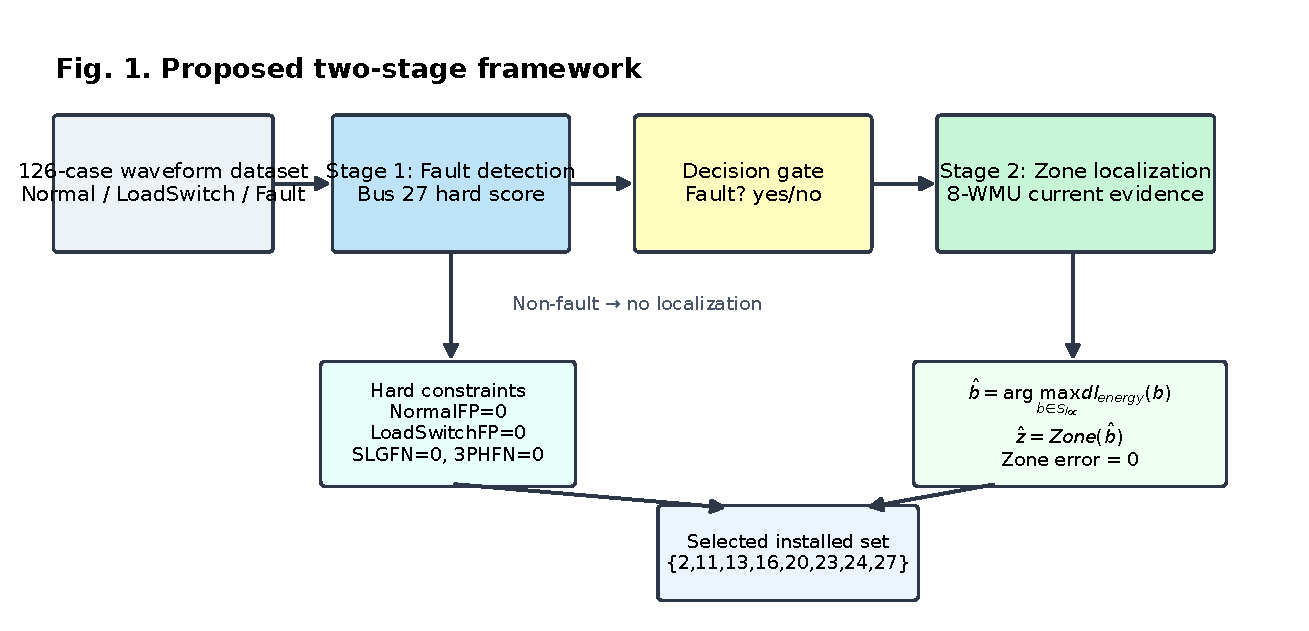
\includegraphics[width=0.95\textwidth]{Fig1_proposed_two_stage_framework.pdf}
\caption{Proposed two-stage framework. Stage 1 performs hard-constrained fault detection using Bus 27 as the detection anchor. Stage 2 performs current-disturbance-based zone localization using the selected eight-WMU localization set.}
\label{fig:framework}
\end{figure*}

Let $\mathcal{B}=\{1,2,\ldots,30\}$ denote the IEEE 30-bus candidate bus set. Each event case $i$ is assigned a binary label
\begin{equation}
y_i\in\{0,1\},
\end{equation}
where $y_i=0$ denotes a non-fault case, including normal operation and LoadSwitch disturbances, and $y_i=1$ denotes a fault case, including SLG and three-phase faults. For fault cases, the true faulted bus is denoted by $b_i$, and the corresponding topology zone is
\begin{equation}
z_i=Z(b_i),
\end{equation}
where $Z(\cdot)$ maps each bus to its predefined topology zone.

The design motivation is that the WMU subset that is sufficient for fault/non-fault detection is not necessarily sufficient for location identification. The final system therefore uses
\begin{equation}
S_{det}=\{27\}
\end{equation}
for detection and
\begin{equation}
S_{loc}=\{2,11,13,16,20,23,24,27\}
\end{equation}
for localization.

\section{Stage 1: Hard-Constrained Fault Detection}

\subsection{Event Label Definition}

Let $e_i$ denote the event type of case $i$. The non-fault and fault event sets are defined as
\begin{equation}
\mathcal{C}_0=\{\mathrm{SSO\_Normal},\mathrm{SSO\_LoadSwitch}\},
\end{equation}
\begin{equation}
\mathcal{C}_1=\{\mathrm{SSO\_SLG\_Fault},\mathrm{SSO\_ThreePhase\_Fault}\}.
\end{equation}
The binary fault label is
\begin{equation}
y_i=\begin{cases}
0, & e_i\in\mathcal{C}_0,\\
1, & e_i\in\mathcal{C}_1.
\end{cases}
\end{equation}
This binary mapping follows protection-oriented transient studies in which load switching is treated as a normal or non-fault disturbance rather than as a fault.

\subsection{Bus-Wise Normalization and Evidence Features}

Let $x_{i,b,f}$ be the raw value of feature $f$ for case $i$ at observed bus $b$. For each bus and feature, the 5th and 95th percentiles are computed as
\begin{equation}
q_{b,f}^{0.05}=Q_{0.05}(\{x_{i,b,f}:i\in\mathcal{I}\}),
\end{equation}
\begin{equation}
q_{b,f}^{0.95}=Q_{0.95}(\{x_{i,b,f}:i\in\mathcal{I}\}).
\end{equation}
The normalized feature is
\begin{equation}
\tilde{x}_{i,b,f}=\mathrm{clip}_{[0,1]}\left(\frac{x_{i,b,f}-q_{b,f}^{0.05}}{\max(q_{b,f}^{0.95}-q_{b,f}^{0.05},\epsilon)}\right),\quad \epsilon=10^{-12}.
\end{equation}
This normalization is performed per observed bus, not globally, to prevent buses with naturally larger absolute waveform magnitudes from dominating the placement score.

The fault evidence feature set includes voltage/current disturbance energy,
voltage sag, RMS-current jump, sequence/unbalance ratios, and apparent-
impedance change features. In compact form,
\begin{equation}
\mathcal{F}_{fault}=\{f^{fault}_1,f^{fault}_2,\ldots,f^{fault}_{13}\}.
\end{equation}
These features reflect voltage sag, current disturbance, sequence imbalance, and apparent-impedance change.

LoadSwitch evidence is based on the 67--77 Hz voltage cycle-difference ratio in three phases:
\begin{align}
\mathcal{F}_{LS}=\{&\mathrm{dV\_E72\_ratio\_A},
\mathrm{dV\_E72\_ratio\_B},\nonumber\\
&\mathrm{dV\_E72\_ratio\_C}\}.
\end{align}

\subsection{Detection Score and Hard Constraints}

For each case and bus, fault evidence is defined as
\begin{equation}
F_{i,b}=\max_{f\in\mathcal{F}_{fault}}\tilde{x}_{i,b,f},
\end{equation}
and LoadSwitch evidence is defined as
\begin{equation}
L_{i,b}=\min_{\phi\in\{A,B,C\}}\tilde{x}_{i,b,\mathrm{dV\_E72\_ratio}_{\phi}}.
\end{equation}
For the detection anchor $b_d$, the score is
\begin{equation}
s_{i,b_d}=F_{i,b_d}-\lambda L_{i,b_d},\quad \lambda=0.5.
\end{equation}
The maximum non-fault score and minimum fault score are
\begin{equation}
M_0(b_d)=\max_{i:y_i=0}s_{i,b_d},\quad m_1(b_d)=\min_{i:y_i=1}s_{i,b_d}.
\end{equation}
The separation margin is
\begin{equation}
\gamma_{det}(b_d)=m_1(b_d)-M_0(b_d).
\end{equation}
If $\gamma_{det}(b_d)>0$, the midpoint threshold is selected:
\begin{equation}
\tau(b_d)=\frac{M_0(b_d)+m_1(b_d)}{2}.
\end{equation}
The predicted label is
\begin{equation}
\hat{y}_i=\mathbb{I}(s_{i,b_d}>\tau).
\end{equation}

A detection anchor is feasible only if
\begin{align}
\mathrm{NormalFP}=0,\quad \mathrm{LoadSwitchFP}=0,\nonumber\\
\mathrm{SLGFN}=0,\quad \mathrm{ThreePhaseFN}=0.
\end{align}
Bus 27 satisfies these hard constraints and provides the detection confusion matrix in Fig.~\ref{fig:detcm}.

\begin{figure}[t]
\centering
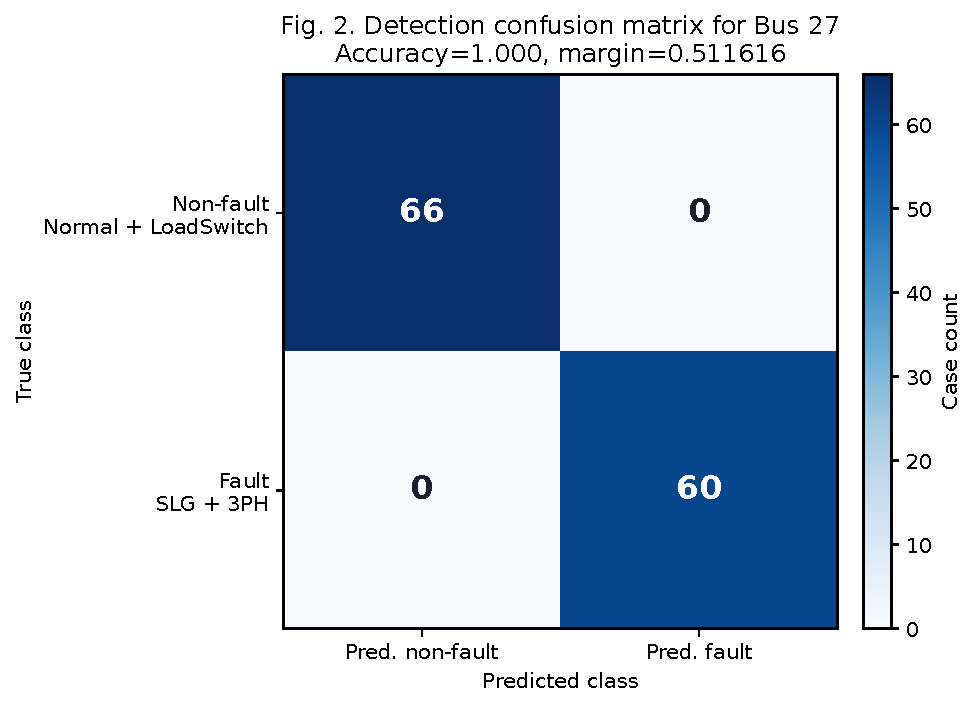
\includegraphics[width=0.95\columnwidth]{Fig2_detection_confusion_matrix_bus27.pdf}
\caption{Detection confusion matrix for Bus 27. The evaluated dataset contains 66 non-fault cases and 60 fault cases, and Bus 27 produces zero evaluated detection errors.}
\label{fig:detcm}
\end{figure}

\section{Stage 2: Current-Disturbance-Based Zone Localization}

\subsection{Argmax Localization Rule}

After a case is classified as a fault, Stage 2 estimates the faulted topology zone. For each fault case $i$ and installed localization WMU $b\in S_{loc}$, the localization stage uses
\begin{equation}
D_{i,b}=dI\_energy_{3ph,max}(i,b).
\end{equation}
The predicted location proxy bus is selected by
\begin{equation}
\hat{b}_i(S_{loc})=\argmaxop_{b\in S_{loc}}D_{i,b}.
\end{equation}
The predicted fault zone is then
\begin{equation}
\hat{z}_i(S_{loc})=Z(\hat{b}_i(S_{loc})).
\end{equation}
This rule is physically interpretable: the installed WMU with the largest current-disturbance energy is treated as a proxy for the faulted region. Fig.~\ref{fig:argmax} illustrates this decision rule.

\begin{figure}[t]
\centering
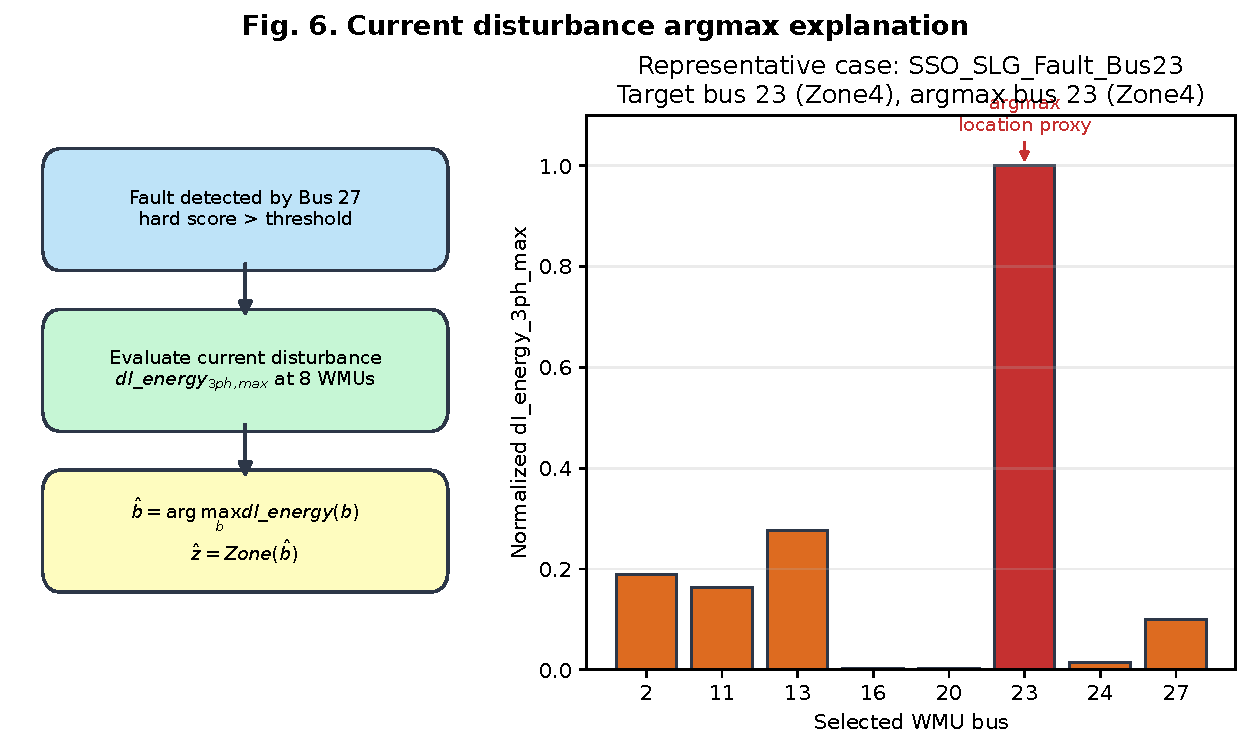
\includegraphics[width=0.98\columnwidth]{Fig6_current_disturbance_argmax_explanation.pdf}
\caption{Current disturbance argmax explanation. After a fault is detected, the localization stage compares $dI\_energy_{3ph,max}$ across the selected WMU buses, chooses the maximum as the location proxy, and maps the proxy bus to a topology zone.}
\label{fig:argmax}
\end{figure}

\subsection{Zone-Localization Constraint}

The zone-localization error for a localization set $S_{loc}$ is defined over the evaluated fault-case set $\mathcal{F}$:
\begin{equation}
\ZoneErr(S_{loc})=\sum_{i\in\mathcal{F}}\mathbb{I}(\hat{z}_i(S_{loc})\neq z_i).
\end{equation}
A localization set is feasible if
\begin{equation}
\ZoneErr(S_{loc})=0.
\end{equation}
The minimum zone-localization placement problem is
\begin{equation}
S^*_{loc}=\argminop_{S\subseteq\mathcal{B}} |S|
\end{equation}
subject to
\begin{equation}
\ZoneErr(S)=0.
\end{equation}
The term minimum is therefore defined with respect to the specified dataset, zone definition, current-disturbance feature, and argmax rule.

\subsection{Exhaustive Search}

The exhaustive search evaluates all candidate WMU subsets in increasing order of cardinality. For each subset size $k$, all combinations $S\subseteq\mathcal{B}$ satisfying $|S|=k$ are tested. The search terminates at the first $k$ for which at least one subset satisfies zero zone error. The search result is shown in Fig.~\ref{fig:mink}. No zero-error subset exists for $k=1,2,\ldots,7$. At $k=8$, five zero-error subsets are found among 5,852,925 evaluated combinations. Thus,
\begin{equation}
k^*_{zone}=8.
\end{equation}

\begin{figure}[t]
\centering
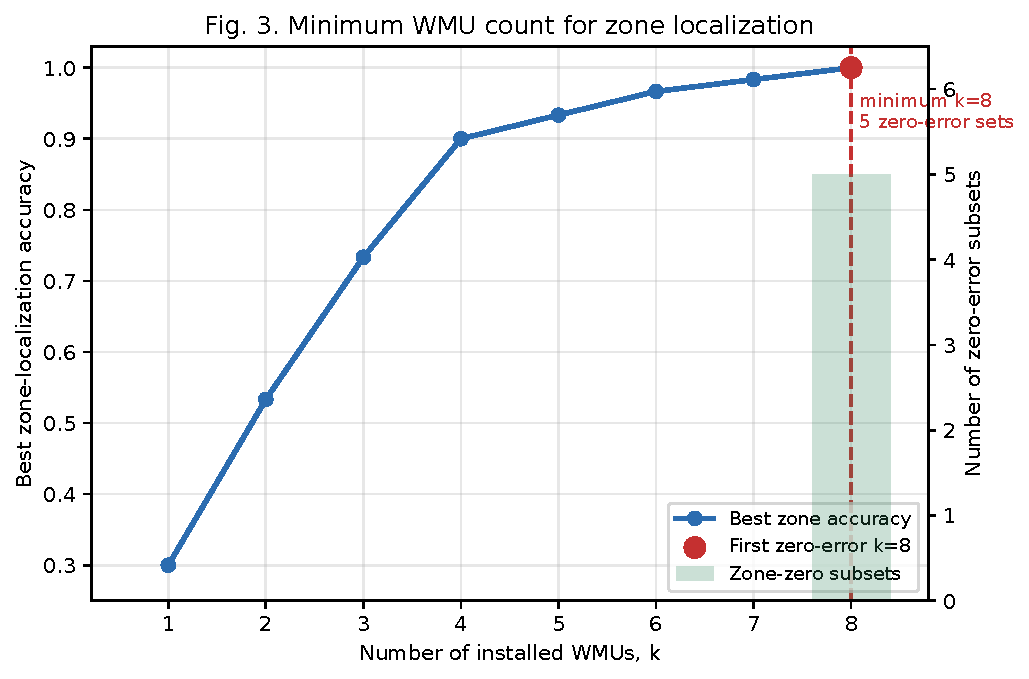
\includegraphics[width=0.98\columnwidth]{Fig3_minimum_wmu_count_zone_localization.pdf}
\caption{Minimum WMU count for zone localization. Exhaustive subset search shows that the first zero-zone-error solutions occur at $k=8$.}
\label{fig:mink}
\end{figure}

Among the five feasible eight-WMU subsets, this paper selects
\begin{equation}
S^*_{loc}=\{2,11,13,16,20,23,24,27\}.
\end{equation}
This set is selected because it satisfies the zero zone-localization constraint and includes Bus 27, the detection anchor identified in Stage 1. Fig.~\ref{fig:network} shows the selected placement on the IEEE 30-bus topology, and Fig.~\ref{fig:zonecm} shows the zone-localization confusion matrix.

\begin{figure}[t]
\centering
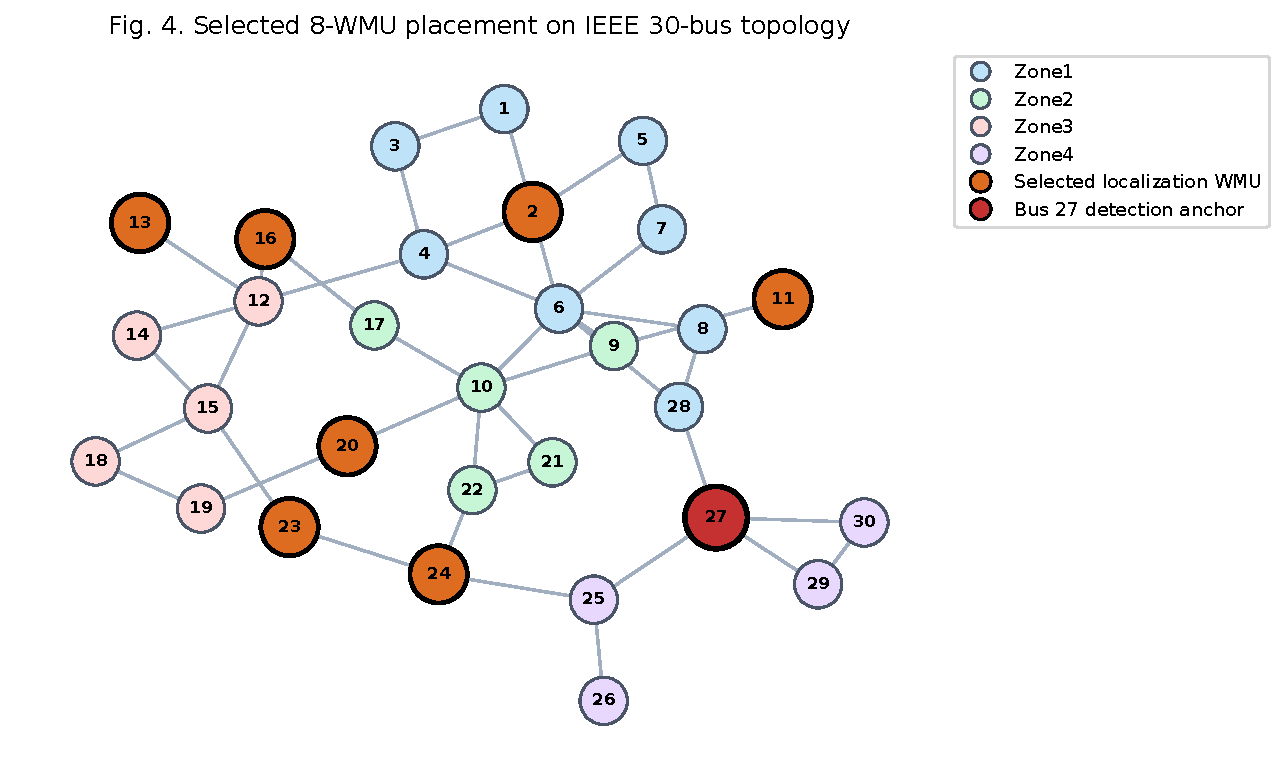
\includegraphics[width=0.98\columnwidth]{Fig4_selected_8wmu_network_map.pdf}
\caption{Selected eight-WMU placement on the IEEE 30-bus topology. The final localization set is $\{2,11,13,16,20,23,24,27\}$, and Bus 27 is also the detection anchor.}
\label{fig:network}
\end{figure}

\begin{figure}[t]
\centering
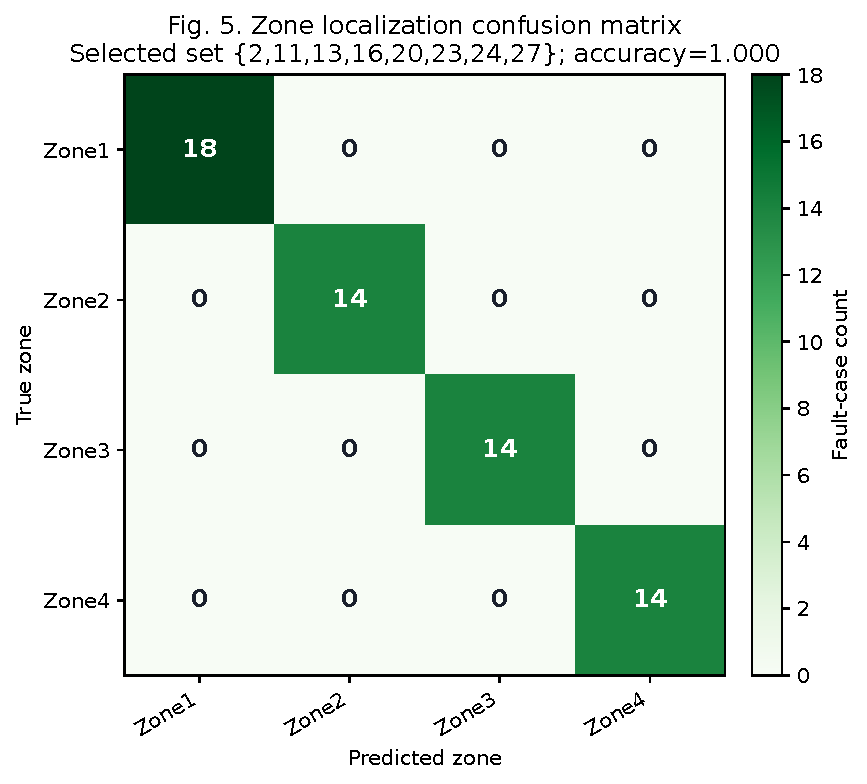
\includegraphics[width=0.95\columnwidth]{Fig5_zone_localization_confusion_matrix.pdf}
\caption{Zone localization confusion matrix for the selected eight-WMU set. The selected placement achieves zero zone-localization error over the 60 evaluated fault cases.}
\label{fig:zonecm}
\end{figure}

\section{Case Study}

\subsection{Test System and Dataset}

The case study uses a modified IEEE 30-bus system. An IBR-like 25 Hz SSO background is included in all event classes to reflect oscillatory monitoring conditions associated with weak-grid IBR interactions. The dataset contains 126 deterministic simulation cases, as summarized in Table~\ref{tab:dataset}.

\begin{table}[t]
\caption{Combined Dataset Composition}
\label{tab:dataset}
\centering
\begin{tabular}{llcc}
\toprule
Event type & Magnitude & Cases & Binary class\\
\midrule
SSO\_Normal & -- & 3 & Non-fault\\
SSO\_LoadSwitch & 5\% & 21 & Non-fault\\
SSO\_LoadSwitch & 15\% & 21 & Non-fault\\
SSO\_LoadSwitch & 30\% & 21 & Non-fault\\
SSO\_SLG\_Fault & -- & 30 & Fault\\
SSO\_ThreePhase\_Fault & -- & 30 & Fault\\
\midrule
Total & -- & 126 & --\\
\bottomrule
\end{tabular}
\end{table}

The dataset includes 66 non-fault cases and 60 fault cases. The LoadSwitch cases are divided into 5\%, 15\%, and 30\% magnitudes to test whether a selected placement remains feasible as non-fault switching severity changes.

\subsection{Detection Result}

The Bus 27 detection anchor yields zero evaluated false positives and zero evaluated false negatives. Table~\ref{tab:bus27} summarizes the result. The score separation satisfies
\begin{equation}
-0.038596 < 0.217212 < 0.473020,
\end{equation}
where $-0.038596$ is the largest non-fault score, $0.473020$ is the smallest fault score, and $0.217212$ is the threshold. The resulting margin is $0.511616$.

\begin{table}[t]
\caption{Selected Bus 27 Detection Performance}
\label{tab:bus27}
\centering
\begin{tabular}{lc}
\toprule
Metric & Value\\
\midrule
Selected detection WMU & Bus 27\\
NormalFP & 0\\
LoadSwitchFP & 0\\
SLGFN & 0\\
ThreePhaseFN & 0\\
TotalFP / TotalFN & 0 / 0\\
Binary accuracy & 1.000\\
Non-fault max score & -0.038596\\
Fault min score & 0.473020\\
Threshold & 0.217212\\
Fault-score margin & 0.511616\\
\bottomrule
\end{tabular}
\end{table}

\subsection{Localization Result}

The localization exhaustive search result is summarized in Table~\ref{tab:locsearch}. The best zone accuracy increases with $k$, but a zero-zone-error subset does not exist until $k=8$.

\begin{table}[t]
\caption{Exhaustive Zone-Localization Search Summary}
\label{tab:locsearch}
\centering
\begin{tabular}{cccc}
\toprule
$k$ & Total subsets & Zero-error subsets & Best accuracy\\
\midrule
1 & 30 & 0 & 0.5000\\
2 & 435 & 0 & 0.7167\\
3 & 4,060 & 0 & 0.8333\\
4 & 27,405 & 0 & 0.9000\\
5 & 142,506 & 0 & 0.9500\\
6 & 593,775 & 0 & 0.9667\\
7 & 2,035,800 & 0 & 0.9833\\
8 & 5,852,925 & 5 & 1.0000\\
\bottomrule
\end{tabular}
\end{table}

The selected localization set $\{2,11,13,16,20,23,24,27\}$ achieves zero zone-localization error over all evaluated fault cases. Because the set includes the Bus 27 detection anchor, the final two-stage installation does not require a separate detection-only sensor outside the localization placement.

\section{Discussion}

The proposed result highlights an important distinction between fault detection and fault localization. Under the evaluated hard constraints, a single WMU at Bus 27 is sufficient for binary fault detection. However, localizing the detected fault to the correct topology zone requires a larger sensor set. The exhaustive search shows that no subset with $k\leq 7$ can satisfy zero zone error under the specified feature, zone definition, and argmax rule. The first feasible localization solutions occur at $k=8$.

This distinction prevents an overstatement of the detection-only result. A single WMU should not be claimed to solve all monitoring objectives merely because it can separate fault and non-fault cases in the evaluated dataset. Instead, the proposed two-stage architecture explicitly quantifies the additional WMU requirement needed to support fault-zone identification.

The result should also be interpreted with caution. The dataset is deterministic and limited in operating-condition diversity. Normal cases are limited, stochastic load variation is not included, and the SSO background is fixed. Measurement noise, missing channels, communication delay, synchronization error, fault resistance variation, inception-angle variation, and other uncertainties should be included in future validation.

\section{Conclusion}

This paper proposed a two-stage hard-constrained WMU placement framework for fault detection and zone localization under IBR-like oscillatory background conditions. Stage 1 uses Bus 27 as a detection anchor and achieves zero evaluated NormalFP, LoadSwitchFP, SLGFN, and ThreePhaseFN with a fault-score margin of 0.511616. Stage 2 performs current-disturbance-based localization using an argmax rule over the installed WMU set. Exhaustive search shows that zero-error zone localization first becomes feasible at $k=8$, and the selected final placement is $\{2,11,13,16,20,23,24,27\}$. The study demonstrates that the minimum WMU requirement depends on the monitoring objective: one WMU is sufficient for the evaluated detection task, whereas eight WMUs are required for zero-error zone localization under the specified formulation.

Future work should expand the dataset by varying SSO frequency, SSO amplitude, damping, load level, fault resistance, fault inception angle, measurement noise, missing data, and synchronization error. The hard-constrained framework can also be extended toward train/validation/test thresholding, N-1 sensor contingency constraints, and joint detection--classification--localization placement.

\bibliographystyle{IEEEtran}
\bibliography{references}

\end{document}
